\documentclass[NET,english,aspectratio=169]{tumbeamer}

%settings
\usepackage[utf8]{inputenc}
\usepackage{pgfplotstable}
\usepackage{marvosym}
\usepackage{filecontents}
\usepackage{packages}
\usepackage{beamermods}

\usepackage[backend=bibtex, style=ieee]{biblatex}

\usepackage{csquotes}

\usetikzlibrary{calc}
\usetikzlibrary{arrows.meta}


% For lecture mode (use package option 'lecture'):
%\lecture[GRNVS]{Grundlagen Rechnernetze und Verteilte Systeme}
%\module{IN0010}
%\semester{SoSe\,2016}
%\assistants{Johannes Naab, Stephan Günther, Maurice Leclaire}

\usepackage{pgfplots}
\pgfplotsset{compat=newest}
\usepackage{tumcolor}
\usepackage{tumcolors}
\usepackage{textpos}


\usepackage{pgfpages}
\usepackage{ifthen}
% ============================================================================
% jobname solution
% ============================================================================
\newif\ifsolution%
\ifthenelse{\equal{\detokenize{notes}}{\jobname}}{%
\setbeameroption{show notes on second screen=bottom}
\setbeamercolor{note page}{bg=white, fg=black}
\setbeamercolor{note title}{bg=white!95!black, fg=black}
}{
}

%\xdefinecolor{orange}{cmyk}{0,0.65,0.95,0} 
%\xdefinecolor{dblue}{cmyk}{1,0.54,0.04,0.19}
%\xdefinecolor{blue}{cmyk}{1,0.43,0,0}  
%\xdefinecolor{lblue}{cmyk}{0.65,0.19,0.01,0.04}
%\xdefinecolor{green} {cmyk}{0.35,0,1,0.2} 
%xdefinecolor{yellow}{rgb}{1.00,0.71,0.00} 
%\colorlet{lgtorange}{orange!20} 
%\colorlet{lgtdblue}{dblue!20} 
%\colorlet{lgtblue}{blue!20} 
%\colorlet{lgtlblue}{lblue!20} 
%colorlet{lgtgreen}{green!20} 
%\colorlet{lgtyellow}{yellow!20}

\newcommand\Wider[2][3em]{%
\makebox[\linewidth][c]{%
  \begin{minipage}{\dimexpr\textwidth+#1\relax}
  \raggedright#2
  \end{minipage}%
  }%
}
\usepackage{cancel}
\usepackage{minted}


\addbibresource{lit.bib}


% For beamer mode (default):
\author{Paul Emmerich}
\title{Demystifying Network Cards}
\date{December 27, 2017}

\begin{document}

\begin{frame}{About me}
\begin{tikzpicture}[remember picture,overlay]
    \node[xshift=-2.5cm,yshift=-3cm] at (current page.north east) {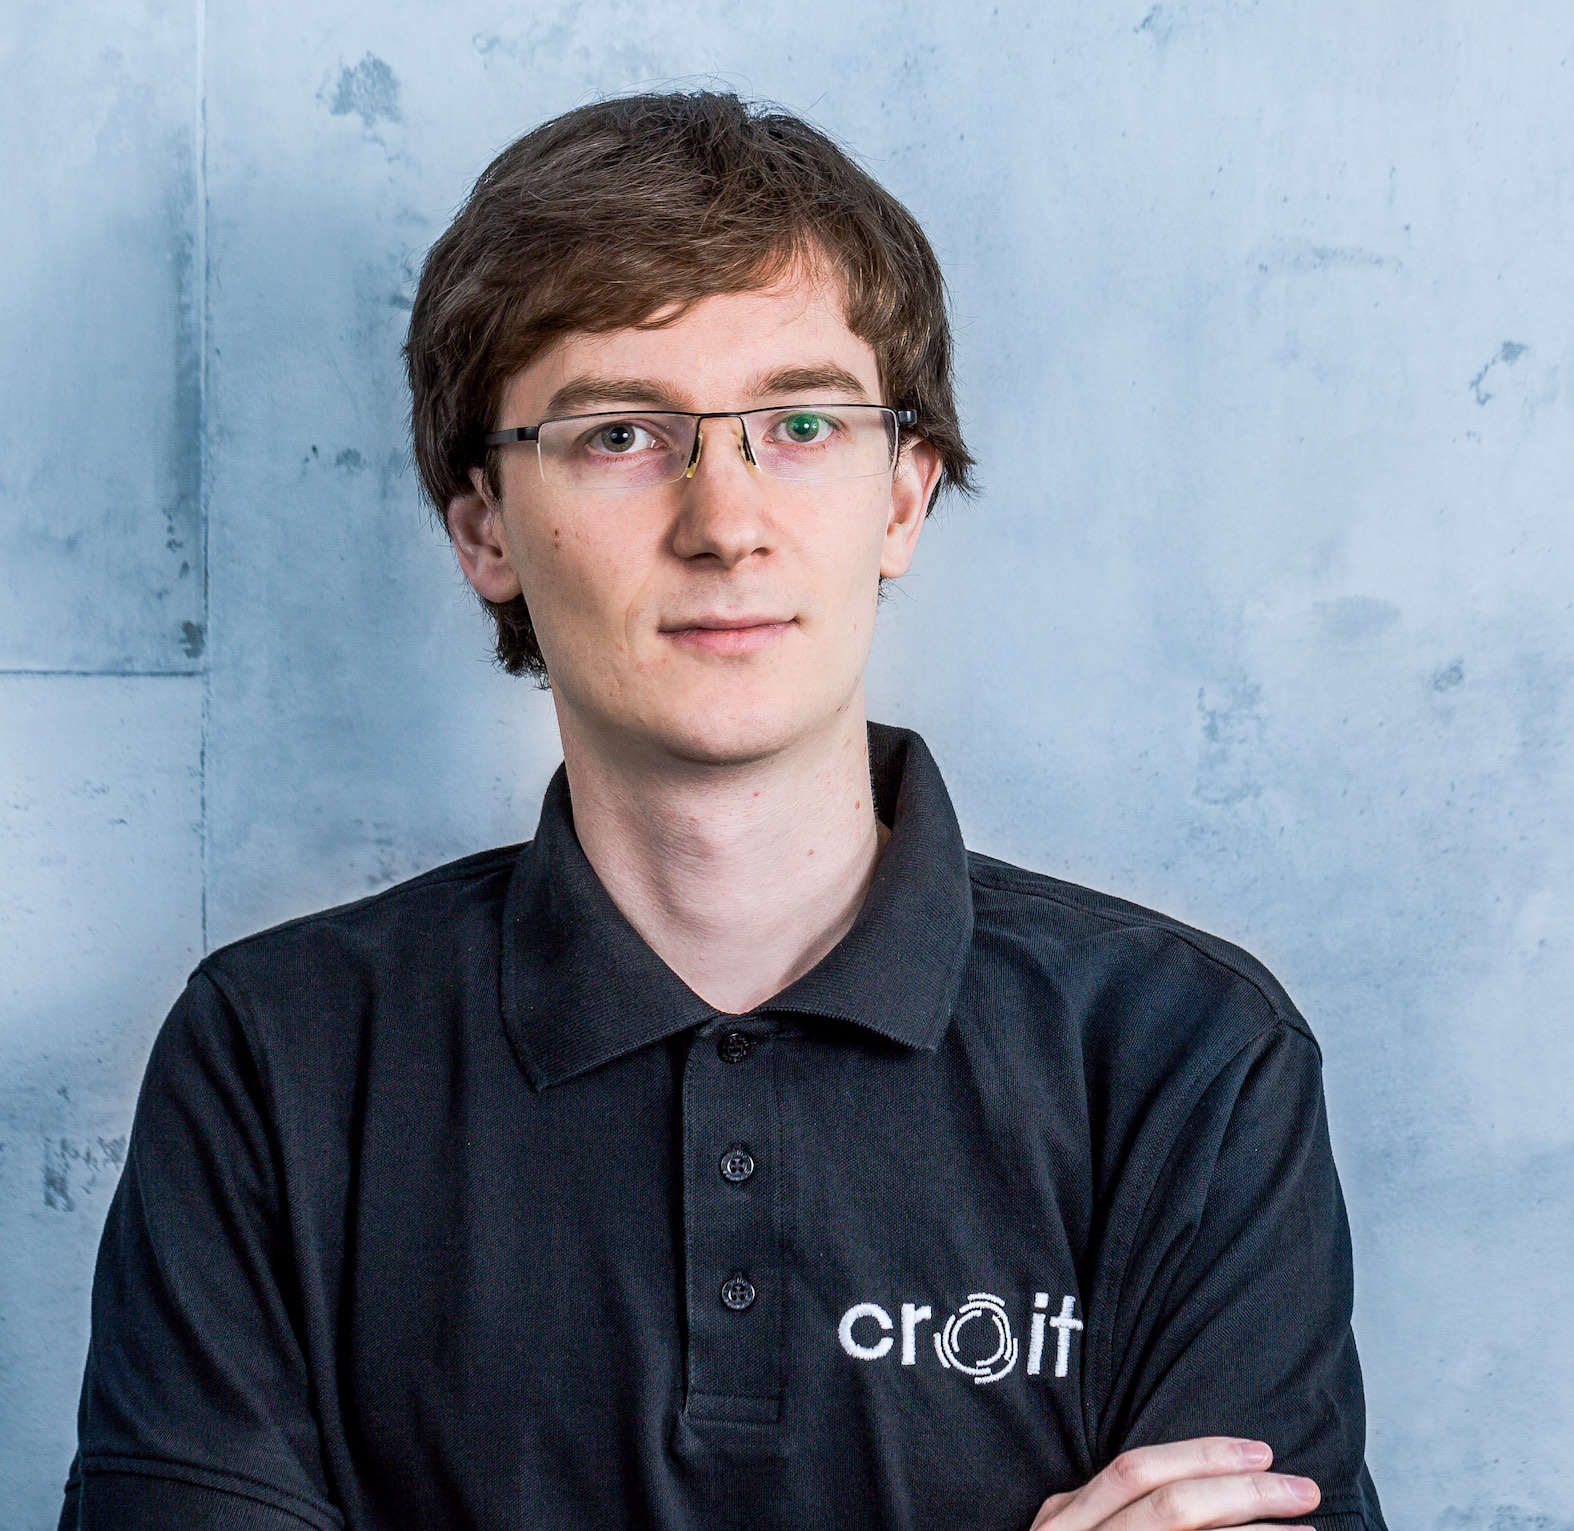
\includegraphics[width=0.2\textwidth]{pics/me.jpg}};
\end{tikzpicture}
\begin{itemize}
\item PhD student at Technical University of Munich
\item Researching performance of software packet processing systems
\item Mostly working on my packet generator MoonGen
\begin{itemize}
\item<2-> Lightning talk about packet generators on Saturday
\end{itemize}
\end{itemize}
\pause
\begin{tikzpicture}[remember picture,overlay]
    \node[xshift=-2.5cm,yshift=2cm] at (current page.south east) {
\includegraphics[width=0.2\textwidth]{pics/moongenlogo.pdf}};
\end{tikzpicture}
\end{frame}

%\begin{frame}{Network Interface Card (NIC)}
%\centering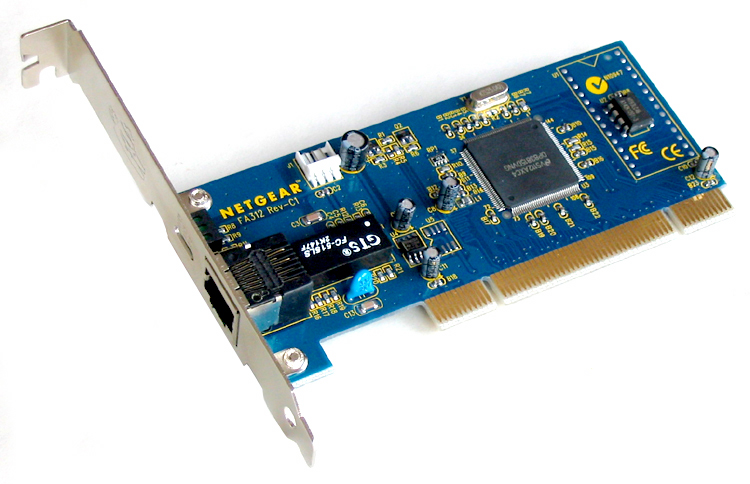
\includegraphics[width=0.66\textwidth]{pics/nic1}
%\end{frame}

\begin{frame}{Network Interface Card (NIC)}
\centering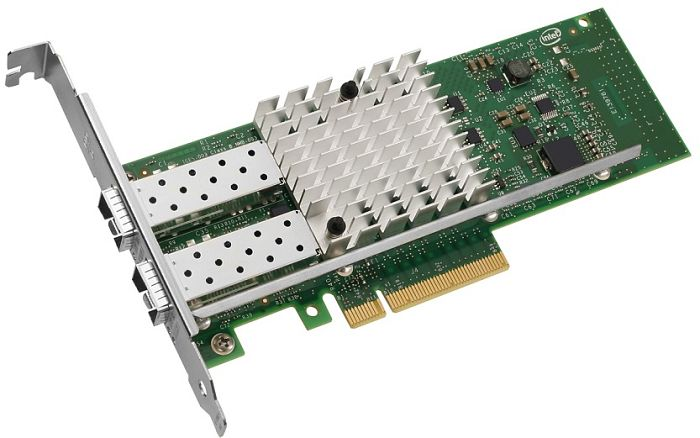
\includegraphics[width=0.66\textwidth]{pics/nic2}
\end{frame}

\begin{frame}{Network Interface Card (NIC)}
\centering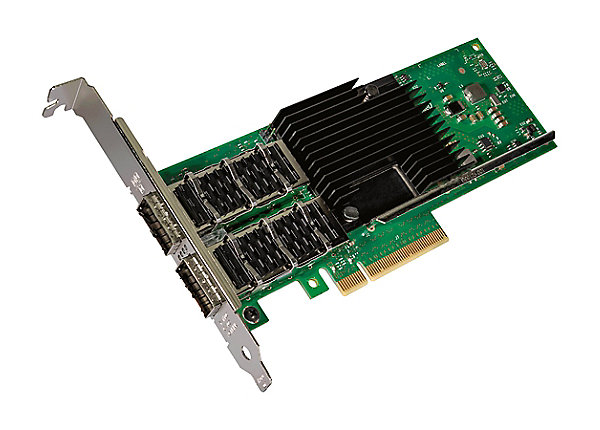
\includegraphics[width=0.66\textwidth]{pics/nic3}
\end{frame}


\begin{frame}{What I care about}
\centering\begin{tikzpicture}[scale=1.35]
	\foreach \x in {1,2,...,7} {
		\pgfmathparse{40 - \x*5}\let\layershade\pgfmathresult
		\pgfmathparse{\x/2}\let\y\pgfmathresult
		\def\layercolor{TUMDarkerBlue}
		\draw[line width=.5pt,fill=\layercolor!\layershade]
			(0,\y) rectangle ($(4,\y+0.5)$);

	}
	\foreach \x in {1,2,...,7} {
		\node at (0.17,0.25+\x*0.5) {\fontsize{5}{6}\selectfont\bf \x};
	}
	\node at (2,0.75) {\fontsize{7}{8}\selectfont Physical};
	\node at (2,1.25) {\fontsize{7}{8}\selectfont Data Link};
	\node at (2,1.75) {\fontsize{7}{8}\selectfont Network};
	\node at (2,2.25) {\fontsize{7}{8}\selectfont \cancel{Transport}};
	\node at (2,2.75) {\fontsize{7}{8}\selectfont \cancel{Session}};
	\node at (2,3.25) {\fontsize{7}{8}\selectfont \cancel{Presentation}};
	\node at (2,3.75) {\fontsize{7}{8}\selectfont \cancel{Application}};
\end{tikzpicture}
\end{frame}


\begin{frame}{Not all apps run on top of HTTP}
Lots of network functionality is moving from specialized hardware to software:
\begin{itemize}
\item Routers
\item (Virtual) Switches
\item Firewalls
\item Middleboxes
\end{itemize}
Buzzwords: Network Function Virtualization, Service Function Chaining
\end{frame}

\begin{frame}{Example application}
\centering\includestandalone{figures/softwarearch-simple}
\end{frame}


\begin{frame}{Normal applications}
\centering\includestandalone{figures/softwarearch-classic}
\end{frame}

\begin{frame}{What it really looks like}
\centering\includestandalone{figures/softwarearch-dragons}
\end{frame}

\begin{frame}{Performance}
\begin{itemize}
\item Packets per second on a 10\,Gbit/s link: up to \emph{14.88\,Mpps}
\item<2-> Packets per second on a 100\,Gbit/s link: up to \emph{148.8\,Mpps}
\item<3-> Clock cycles per packet on a 3\,GHz CPU with 14.88\,Mpps: $\approx 200$ cycles
\item<3-> Typical performance target: $\approx$ 5 to 10\,Mpps per CPU core for simple forwarding
\end{itemize}
\end{frame}

\begin{frame}{Performance: User space app}
\begin{itemize}
\item<1-> Typical performance target: $\approx$ 5 to 10\,Mpps per CPU core for simple forwarding
\item<1-> 5 to 10\,Mpps $=$ \emph{300 to 600 cycles} per packet at 3\,GHz
\vspace{1em}
\item<2-> Time to cross the user space boundary: very very long
\vspace{1em}
\item<3-> Single-core forwarding performance with sockets: $\approx$ 0.3\,Mpps
\item<3-> Single-core forwarding performance with libpcap: $\approx$ 1\,Mpps
%\item Latency of a typical hardware switch: $\le 1\,\mu s$
%\item Latency of a hardware switch: $\le 1\,\mu s$
\end{itemize}
\end{frame}

%\begin{frame}{Performance dragons?}
%\centering\includestandalone{figures/softwarearch-dragons}
%\end{frame}

\begin{frame}{Move the application into the kernel}
\centering\includestandalone{figures/softwarearch-kernel}
\end{frame}

\begin{frame}{Move the application into the kernel}
New problems:
\begin{itemize}
\item Cumbersome to develop
\item Usual kernel restrictions (e.g., C as programming language)
\item Application can (and will) crash the kernel
\end{itemize}
\end{frame}

\begin{frame}{Performance: Kernel app}
\begin{itemize}
\item<1-> Typical performance target: $\approx$ 5 to 10\,Mpps per CPU core for simple forwarding
\item<1-> 5 to 10\,Mpps $=$ \emph{300 to 600 cycles} per packet at 3\,GHz
\vspace{1em}
\item<2-> Time to receive a packet in the Linux kernel: $\approx \emph{500}$ \emph{cycles}
\item<3-> Time to send a packet in the Linux kernel: $\approx \emph{440}$ \emph{cycles}
\item<4-> Time to allocate, initialize, and free a \texttt{sk\_buff} in the Linux kernel: $\approx \emph{400}$ \emph{cycles}
\vspace{1em}
\item<5-> Single-core forwarding performance with Open vSwitch: $\approx$ 2\,Mpps
\item<5-> Hottest topic in the Linux kernel: XDP, which fixes some of these problems
\end{itemize}
\end{frame}


\begin{frame}{Do more in user space?}
\centering\includestandalone{figures/softwarearch-moreuserspace}
\end{frame}

\begin{frame}{User space packet processing frameworks}
Examples for such frameworks
\begin{itemize}
\item netmap
\item PF\_RING ZC
\item pfq
\end{itemize}
\end{frame}

\begin{frame}{Problems}
\begin{itemize}
\item Non-standard API, custom kernel module required
\item Most frameworks require patched drivers
\item Exclusive access to the NIC for one application
\item No access to the usual kernel features
\begin{itemize}
\item Limited support for kernel integration in netmap
\end{itemize}
\item Poor support for hardware offloading features of NICs
\item Framework needs explicit support for each NIC, limited to a few NICs
\end{itemize}
\end{frame}

\begin{frame}{Do even more in user space?}
\centering\includestandalone{figures/softwarearch-fulluserspace}
\end{frame}

\begin{frame}{User space driver frameworks}
Examples for such frameworks
\begin{itemize}
\item DPDK
\item Snabb
\end{itemize}
\end{frame}

\begin{frame}{Problems}
\begin{itemize}
\item Non-standard API
\item Exclusive access to the NIC for one application
\item Framework needs explicit support for each NIC model
\begin{itemize}
\item DPDK supports virtually all $\ge$ 10\,Gbit/s NICs
\end{itemize}
\item Limited support for interrupts
\begin{itemize}
\item Interrupts not considered useful at $\ge$ 0.1\,Mpps
\end{itemize}
\item No access to the usual kernel features
\end{itemize}
\end{frame}

\begin{frame}{What has the kernel ever done for us?}
\begin{itemize}
\item<1-> Lots of mature drivers
\item<2-> Protocol implementations that actually work (TCP, ...)
\item<3-> Interrupts (NAPI is quite nice)
\item<3-> Stable user space APIs
\item<3-> Access for multiple applications at the same time
\item<3-> Firewalling, routing, eBPF, XDP, ...
\item<3-> ...and more
\end{itemize}
\end{frame}

\begin{frame}{Are these frameworks fast?}
\begin{itemize}
\item<1-> Typical performance target: $\approx$ 5 to 10\,Mpps per CPU core for simple forwarding
\item<1-> 5 to 10\,Mpps $=$ \emph{300 to 600 cycles} per packet at 3\,GHz
\vspace{1em}
\item<2-> Time to receive a packet in DPDK: $\approx \emph{50}$ \emph{cycles}
\item<2-> Time to send a packet in DPDK: $\approx \emph{50}$ \emph{cycles}
\item<2-> Other user space frameworks play in the same league
\vspace{1em}
\item<2-> Single-core forwarding with Open vSwitch on DPDK: $\approx$ 13\,Mpps (2\,Mpps without)
\item<2-> Performance gains from: batching (typically 16 to 64 packets/batch), reduced memory overhead (no \texttt{sk\_buff})
\end{itemize}
\end{frame}

\begin{frame}{Usage}
Lots of packet processing apps have support for DPDK today:
\begin{itemize}
\item Open vSwitch
\item Vyatta
\item Juniper's vMX
\item Cisco's VPP
\item pfSense (soon)
\end{itemize}
Main reasons: performance and control over hardware features
\end{frame}

\begin{frame}{Can we build our own user space driver?}
Sure, but why?
\begin{itemize}
\item For fun \cancel{and profit}
\item To understand how NIC drivers work
\item To understand how user space packet processing frameworks work
\begin{itemize}
\item Many people see these frameworks as magic black boxes
\item DPDK drivers: $\ge$ 20k lines of code per driver
\end{itemize}
\item How hard can it be?
\item Turns out it's quite easy, I've written my driver Ixy in less than 1000 lines of C
\end{itemize}
\end{frame}

\begin{frame}{Hardware: Intel \texttt{ixgbe} family (10\,Gbit/s)}
\begin{itemize}
\item \texttt{ixgbe} family: 82599ES (aka X520), X540, X550, Xeon D embedded NIC
\item Commonly found in servers or as on-board chips
\item Very good datasheet publicly available
%\vspace{1em}
\item Almost no logic hidden behind black-box firmware
%\item<2-> Black-box firmware contains almost no magic
%\item<2-> Drivers for many newer NICs often just exchanges messages with the firmware
%\item<2-> Here: all hardware features directly exposed to the driver
\end{itemize}
\end{frame}

\begin{frame}{How to build a full user space driver in 4 simple steps}
\begin{itemize}
\item[1.] Unload kernel driver
\item[2.] \texttt{mmap} the PCIe MMIO address space
\item[3.] Figure out physical addresses for DMA
%\item<2->[4.] Write the driver
\item[4.] Write the driver
\end{itemize}
\end{frame}

\newmintinline[ccode]{c}{}
\newmintinline[bashcode]{c}{}

\begin{frame}[fragile=singleslide]{Find the device we want to use}
\begin{Verbatim}[commandchars=\\\{\}]
# lspci
03:00.0 Ethernet controller: Intel Corporation 82599ES 10-Gigabit SFI/SFP+ ...
03:00.1 Ethernet controller: Intel Corporation 82599ES 10-Gigabit SFI/SFP+ ...
\end{Verbatim}
\end{frame}

\begin{frame}[fragile=singleslide]{Find the device we want to use}
\begin{Verbatim}[commandchars=\\\{\}]
# lspci
\textbf{03:00.0} Ethernet controller: Intel Corporation 82599ES 10-Gigabit SFI/SFP+ ...
\textbf{03:00.1} Ethernet controller: Intel Corporation 82599ES 10-Gigabit SFI/SFP+ ...
\end{Verbatim}
\end{frame}

\begin{frame}[fragile=singleslide]{Unload the kernel driver}
\begin{minted}{bash}
echo 0000:03:00.1 > /sys/bus/pci/devices/0000:03:00.1/driver/unbind
\end{minted}
%\begin{itemize}
%\item \ccode{asdf hi}
%\item \ccode|asdf|
%\item \mintinline{c}{hi}
%\end{itemize}
\end{frame}

\begin{frame}[fragile=singleslide]{\texttt{mmap} the PCIe configuration address space from user space}
\begin{minted}[autogobble]{c}
	int fd = open("/sys/bus/pci/devices/0000:03:00.0/resource0", O_RDWR);
	struct stat stat;
	fstat(fd, &stat);
	uint8_t* registers = (uint8_t*) mmap(NULL, stat.st_size, PROT_READ | PROT_WRITE,
	                                     MAP_SHARED, fd, 0);
\end{minted}
%\begin{itemize}
%\item \ccode{asdf hi}
%\item \ccode|asdf|
%\item \mintinline{c}{hi}
%\end{itemize}
\end{frame}

\begin{frame}{Device registers}
\centering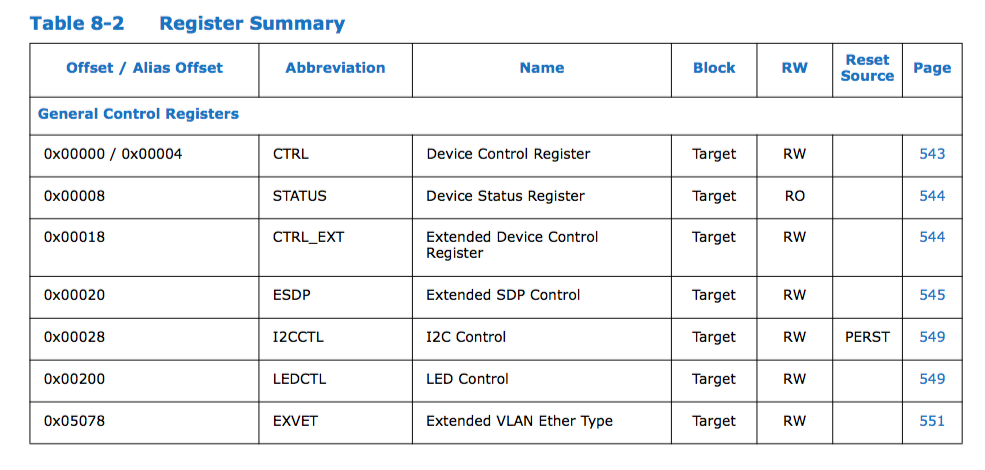
\includegraphics[width=0.75\textwidth]{pics/registers}
\end{frame}

\begin{frame}[fragile=singleslide]{Access registers: LEDs}
\begin{minted}[autogobble]{c}
#define LEDCTL 0x00200
#define LED0_BLINK_OFFS 7

uint32_t leds = *((volatile uint32_t*)(registers + LEDCTL));
*((volatile uint32_t*)(registers + LEDCTL)) = leds | (1 << LED0_BLINK_OFFS);
\end{minted}
\begin{itemize}
\item Memory-mapped IO: all memory accesses go directly to the NIC
\item One of the very few valid uses of \ccode{volatile} in C
\end{itemize}
\end{frame}

\begin{frame}[fragile=singleslide]{How are packets handled?}
\begin{itemize}
\item Packets are transferred via DMA (Direct Memory Access)
\item DMA transfer is initiated by the NIC
\vspace{1em}
\item Packets are transferred via queue interfaces (often called rings)
\item NICs have multiple receive and transmit queues
\begin{itemize}
\item Modern NICs have 128 to 768 queues
\item This is how NICs scale to multiple CPU cores
\item Similar queues are also used in GPUs and NVMe disks
\end{itemize}
\end{itemize}
\end{frame}

\begin{frame}{Rings/Queues}
\begin{itemize}
\item Specific to \texttt{ixgbe}, but most NICs are similar
\item Rings are circular buffers filled with DMA descriptors
\begin{itemize}
\item DMA descriptors are 16 bytes: 8 byte physical pointer, 8 byte metadata
\item Translate virtual addresses to physical addresses using \texttt{/proc/self/pagemap}
\end{itemize}
\vspace{1em}
\item<2-> Queue of DMA descriptors is accessed via DMA
\item<2-> Queue index pointers (head \& tail) available via registers for synchronization
\end{itemize}
\end{frame}

\begin{frame}{Ring memory layout}
\centering\hspace{1cm}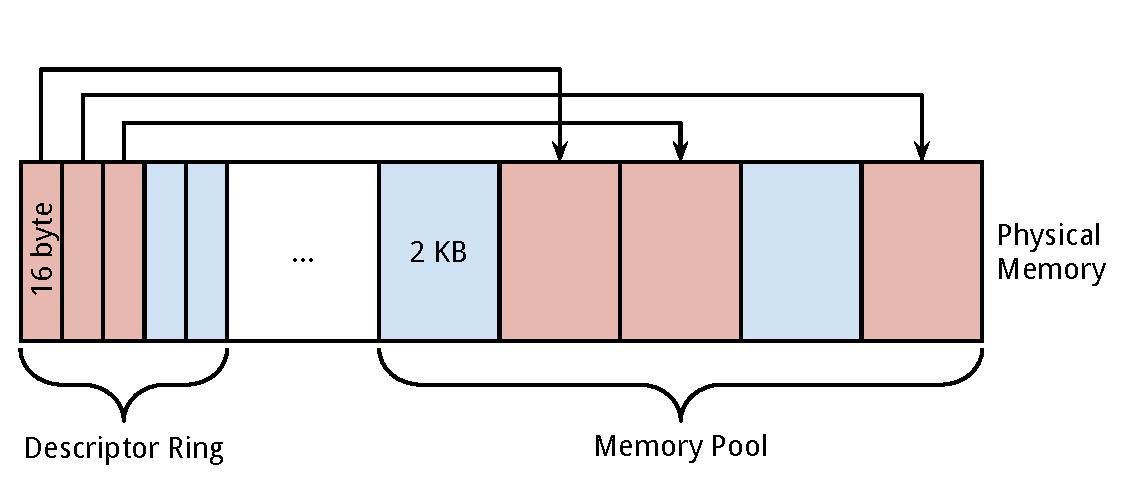
\includegraphics[width=0.75\textwidth]{pics/ring}
\end{frame}

\begin{frame}{Receiving packets}
\begin{itemize}
\item Tell NIC via MMIO the location and size of the ring
\item Fill DMA descriptors with pointers to allocated memory
\end{itemize}
\pause
\begin{itemize}
\item NIC writes a packet via DMA and increments the head pointer
\item NIC also sets a status flag in the DMA descriptor once it's done
\begin{itemize}
\item Checking the status flag is way faster than reading the MMIO-mapped RDH register
\end{itemize}
\pause
\item Periodically poll the status flag
\item Process the packet
\item Reset the DMA descriptor, allocate a new packet or recycle
\item Adjust tail pointer (RDT) register
\end{itemize}
\end{frame}

\begin{frame}{What now?}
\begin{itemize}
\item Transmit rings work the same way
\item There's also a lot of boring initialization code in Ixy
\end{itemize}
\pause
Ideas for things to test with Ixy
\begin{itemize}
\item Performance: why are these frameworks faster than the Kernel?
\item Obscure hardware/offloading features
\item Security features: what about the IOMMU?
\item Other NICs, other programming languages
\end{itemize}
\end{frame}


\begin{frame}{Conclusion: Check out ixy}
\centering \qrcode[height=3cm]{https://github.com/emmericp/ixy}
\begin{itemize}
\item Check out ixy on GitHub: \url{https://github.com/emmericp/ixy} (BSD license)
\item $\le$ 1000 lines of C code for the full framework
\begin{itemize}
	\item C is the lowest common denominator of programming languages
\end{itemize}
\item Drivers are simple: don't be afraid of them. You can write them in any language!
\item No kernel code needed :)
\end{itemize}
%\centering \Huge Q \& A
\end{frame}

\begin{frame}{Backup slides}
\vfill
\centering \huge Backup Slides
\vfill
\end{frame}

\begin{frame}{Linux kernel: past, present, and future}
\emph{Past}
\begin{itemize}
\item Linux 2.4 suffered from problems when moving to 1\,Gbit/s networks
\item One interrupt per packet, servers live-locking under interrupt load
\end{itemize}
\emph{Present}
\begin{itemize}
\item Linux 2.6 added NAPI
\item Dynamic disabling of interrupts, batched receiving
\item Lots of optimizations in the socket API
\end{itemize}
\end{frame}

\begin{frame}{Linux kernel: past, present, and future}
\emph{Present/Future}
\begin{itemize}
\item Hottest Linux networking feature: eXpress Data Path (XDP)
\item Run packet processing code in a fast path in the kernel using eBPF programs
\begin{itemize}
\item Restrictions apply, typically programmed in a restricted subset of C
\end{itemize}
\item Good integration with the kernel
\begin{itemize}
\item Ideal for firewall applications for user space programs on the same host
\end{itemize}
\item<2-> Requires driver support (new memory model) and exclusive NIC access
\item<2-> DPDK supports more NICs than XDP (as of Kernel 4.15)
\item<2-> Work-in-progress, still lacks many features
\end{itemize}
\end{frame}

\begin{frame}[fragile=singleslide]{Setting up a receive ring: code}
\begin{minted}[autogobble]{c}
#define RING_ENTRIES 512
size_t ring_size = RING_ENTRIES * sizeof(struct dma_desc);
struct dma_desc* ring_mem = (struct dma_desc*) malloc(ring_size);
set_reg(RDBAL_0, virt2phy(ring_mem));       // dma descriptor ring location
set_reg(RDBAH_0, virt2phy(ring_mem >> 32)); // dma descriptor ring location
set_reg(RDLEN_0, ring_size);                // dma descriptor size
for (int i = 0; i < RING_ENTRIES; i++) {
	ring_mem[i].dma_ptr = malloc(2048); // NIC will store packet here
}
set_reg(RDH_0, 0);            // head pointer
set_reg(RDT_0, RING_ENTRIES); // tail pointer: rx ring starts out full
\end{minted}
\footnotesize{(Simplified, can't use \ccode{malloc()} because the memory needs to be physically contiguous, real code uses hugetlbfs)}
\end{frame}



%\section{Example Measurements}
%\input{include/measurements}

%\section{P4}
%\input{include/p4}

% Comment out if you do not want a bibliography
%\printbibheading[title={Bibliography},heading=bibnumbered]
%\setbeamertemplate{bibliography item}[text]
%\begin{frame}[allowframebreaks]
%\printbibliography[heading=none]
%\end{frame}

\end{document}

